\paragraph{}
	Pour la séparation backend-frontend nous avons utiliser l'api REST qui nous permet de séparer les action sur la base de donnée et l'interface de l'application web tout en permettant la transmission des donnée grâce au format JSON.
	L'ensemble des requête réaliser si dessous ainsi que leur explication est expliqué dans le chapitre \ref{chap:API}. 
	
\paragraph{}
	La majorité des User Stories sont comparable et applicable au 2 architectures, cependant certaine de c'est User Stories ne sont implémenté qu'uniquement dans la partie Angular. C'est User Stories sont expliqués et illustrer ci-dessous. 

\newpage
\section{User Stories compatible Angular uniquement}
	\paragraph{}
		C'est User Stories on été ajouter part après la création du twig, soit pour faciliter l'exécution d'élément, soit dans le but d'ajouter de nouvelle fonctionnalité. 
	
	\subsection{En tant qu'administrateur, je dois pouvoir créer un type de session}
		\begin{enumerate}
	\item L'administrateur se connecte au site avec ses identifiant. 
	\item Un nouveau bouton de navigation apparait dans la bar de navigation. 
	\item L'administrateur clique sur le bouton \textit{Admin}
	\item Il sélectionne \textit{Type Session} dans le menu déroulant. 
	\item L'administrateur atterris sur la page de gestion des type de sessions. 
	\item Il clique sur \textit{Ajout d'une session +}
	\item Un formulaire apparait et il le remplis avec les bonne information (jour - heure [hh:mm])
	\item Il clique sur \textit{ok} 
\end{enumerate}

\vspace{\baselineskip}
\begin{figure}[h]
	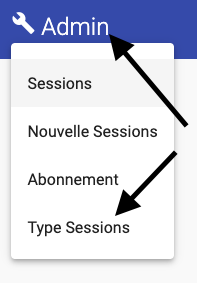
\includegraphics[width=0.3\textwidth,center]{Figures/us12-1}
	\caption{Bouton de navigation de l'administrateur}
\end{figure}

\newpage
\begin{figure}[h]
	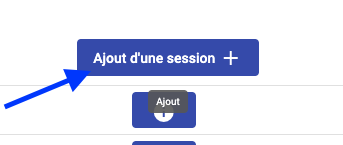
\includegraphics[width=0.5\textwidth,center]{Figures/us12-2}
	\caption{Bouton d'ajout d'un type de session}
\end{figure}

\vspace{\baselineskip}
\begin{figure}[h]
	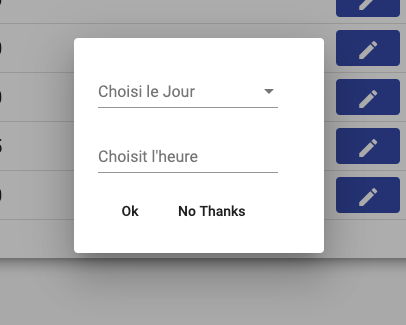
\includegraphics[width=0.5\textwidth,center]{Figures/us12-3}
	\caption{Page d'ajout du type de session}
\end{figure}

\vspace{\baselineskip}
\subsubsection{Gestion des erreurs}
	\begin{itemize}
		\item 2 types de sessions identiques ne peuvent exister, lors de la creation d'un type de session, une vérification se fait et, si le type de session existe deja, une erreur apparait.
		\item Si une erreur apparait durant la création du type de session, elle s'affichera au-dessus du formulaire. 
	\end{itemize}

\newpage
\subsubsection{Diagramme de séquence}
	\begin{figure}[h]
		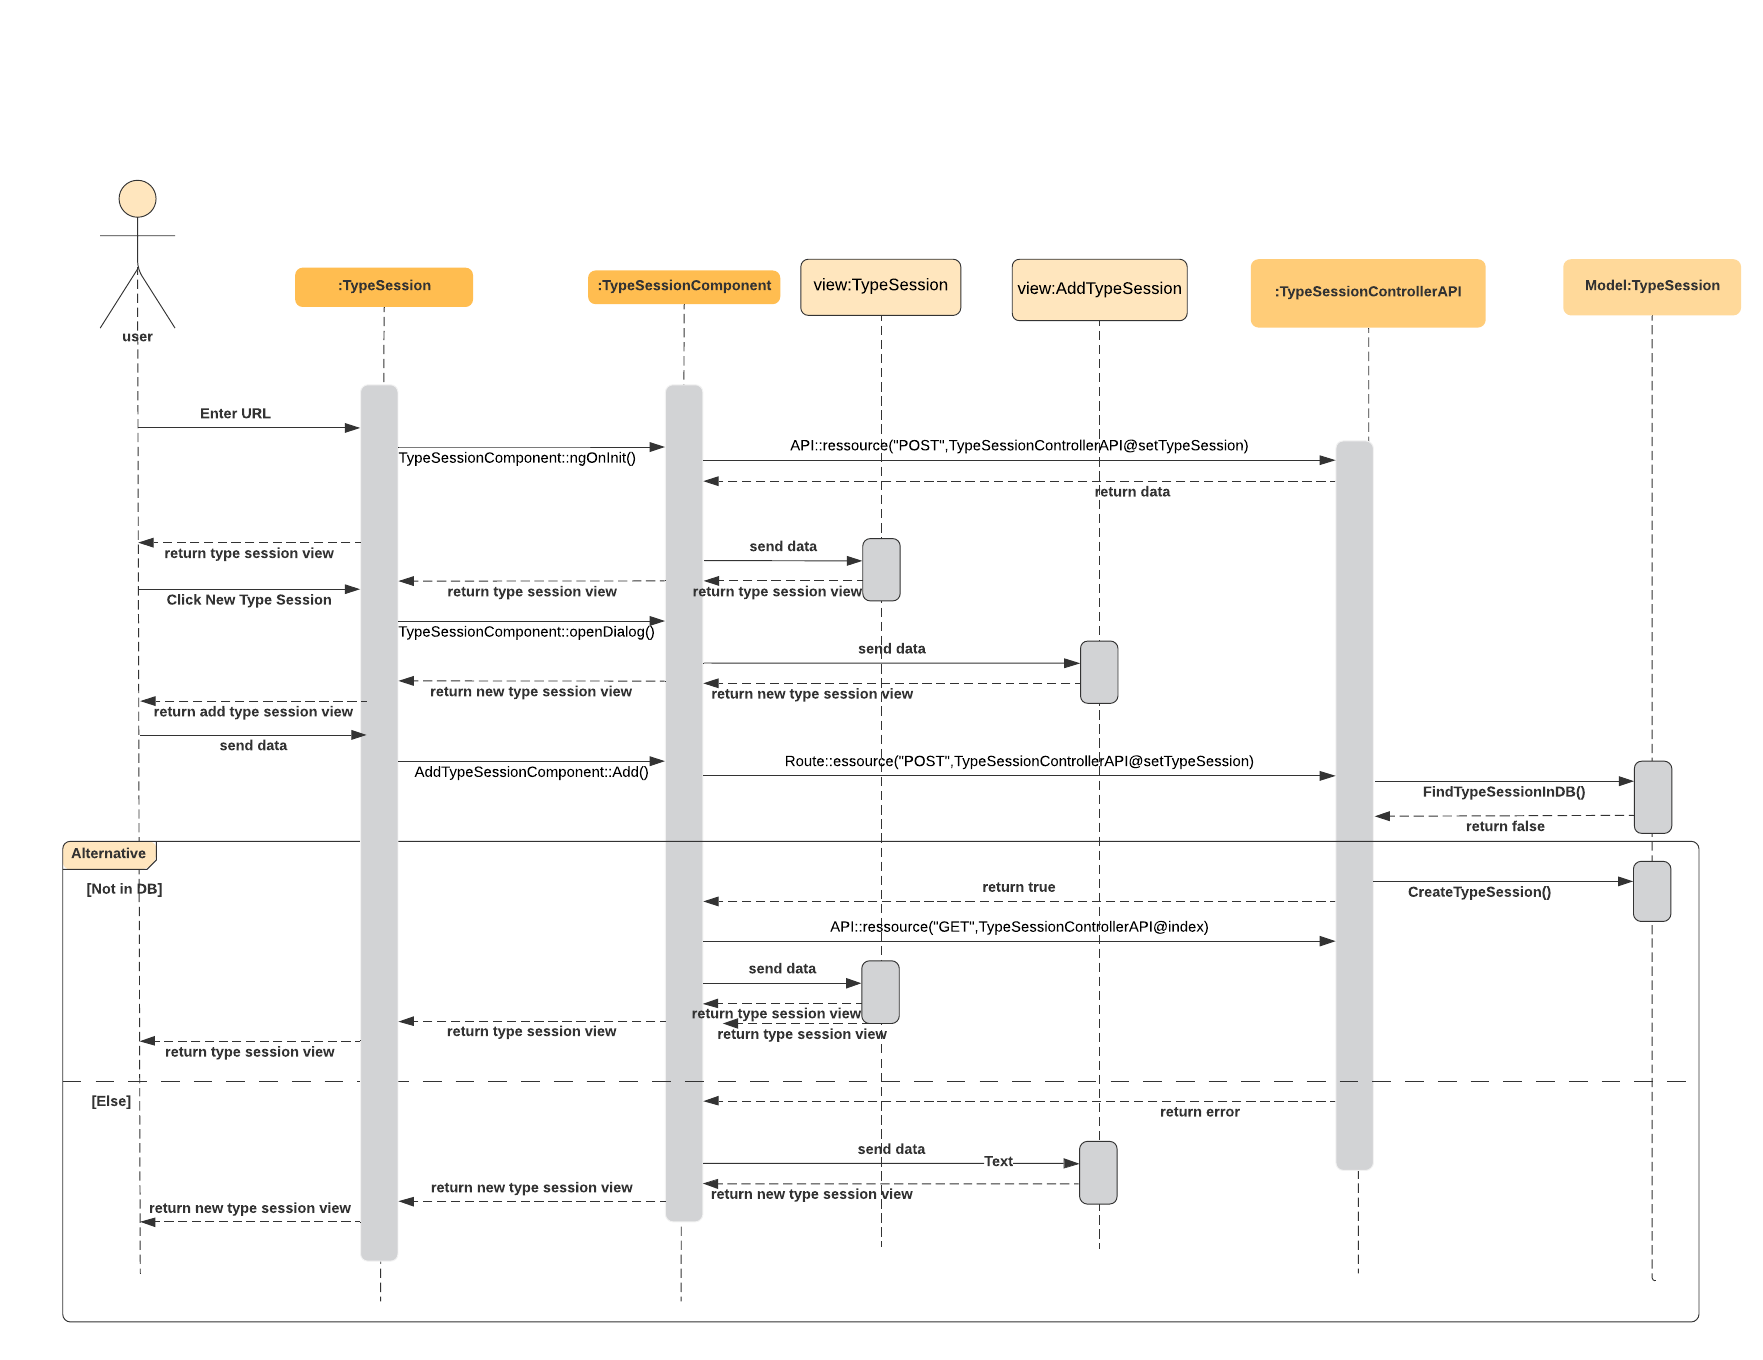
\includegraphics[width=\textwidth,center]{Diagramme/sequence-us12}
		\caption{Diagramme de séquence de l'ajout d'un type de session}
	\end{figure}

\subsubsection{Script concerné}
	\begin{itemize}
		\item \Href{https://github.com/victorsmits/Aquabike/blob/master/backend/src/Controller/API/RegistrationControllerApi.php}{RegistrationControllerApi.php}
		\item \Href{https://github.com/victorsmits/Aquabike/blob/master/backend/src/Entity/TypeSession.php}{TypeSession.php}
		\item \Href{https://github.com/victorsmits/Aquabike/blob/master/frontend/src/app/type-session/add-type-session.component.ts}{add-type-session.component.ts}
		\item \Href{https://github.com/victorsmits/Aquabike/blob/master/frontend/src/app/type-session/add-type-session.component.html}{add-type-session.component.html}
	\end{itemize}

	
	\newpage
	\subsection{En tant qu'administrateur, je veux pouvoir modifier un type de session}
		\begin{enumerate}
	\item L'administrateur se connecte au site avec ses identifiant. 
	\item Un nouveau bouton de navigation apparait dans la bar de navigation. 
	\item L'administrateur clique sur le bouton \textit{Admin}
	\item Il sélectionne \textit{Type Session} dans le menu déroulant. 
	\item L'administrateur atterris sur la page de gestion des type de sessions. 
	\item Il clique sur le bouton edit
	\item Un formulaire apparait et il le remplis avec les bonne information (jour - heure [hh:mm])
	\item Il clique sur \textit{ok} 
\end{enumerate}

\vspace{\baselineskip}
\begin{figure}[h]
	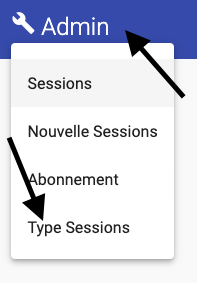
\includegraphics[width=0.4\textwidth,center]{Figures/us13-1}
	\caption{Menu de l'administrateur}
\end{figure}

\newpage
\begin{figure}[h]
	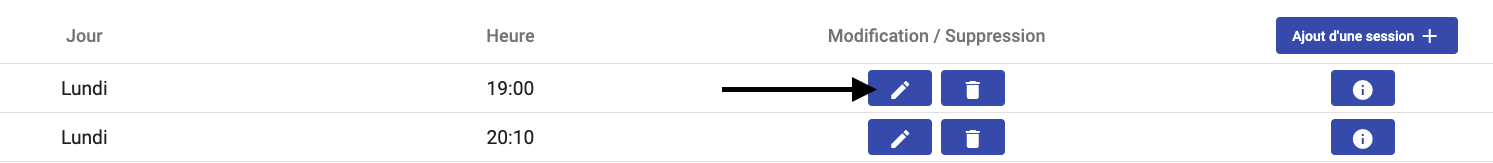
\includegraphics[width=0.9\textwidth,center]{Figures/us13-2}
	\caption{Bouton de modification du type de session}
\end{figure}

\vspace{\baselineskip}
\begin{figure}[h]
	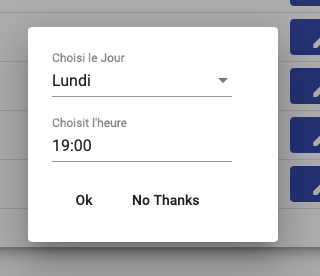
\includegraphics[width=0.4\textwidth,center]{Figures/us13-3}
	\caption{Formulaire de modification du type de session}
\end{figure}

\subsubsection{Gestion des erreurs}
	\paragraph{}
		Chaque type de sessions est unique, si l'administrateur rentre des informations correspondant à un type de sessions deja existant, une erreur apparaitra au dessus du formulaire.
	
	\newpage
	\subsection{En tant qu'administrateur, je veux pouvoir supprimer un type de session}
		\begin{enumerate}
	\item L'administrateur se connecte au site avec ses identifiant. 
	\item Un nouveau bouton de navigation apparait dans la bar de navigation. 
	\item L'administrateur clique sur le bouton \textit{Admin}
	\item Il sélectionne \textit{Type Session} dans le menu déroulant. 
	\item L'administrateur atterris sur la page de gestion des type de sessions. 
	\item Il clique sur le bouton supprimer
	\item Une fenêtre de confirmation apparait. 
	\item Il clique sur \textit{OUI!} 
\end{enumerate}


\begin{figure}[h]
	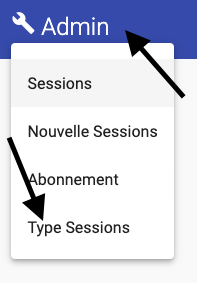
\includegraphics[width=0.4\textwidth,center]{Figures/us13-1}
	\caption{Menu de l'administrateur}
\end{figure}

\vspace{\baselineskip}
\begin{figure}[h]
	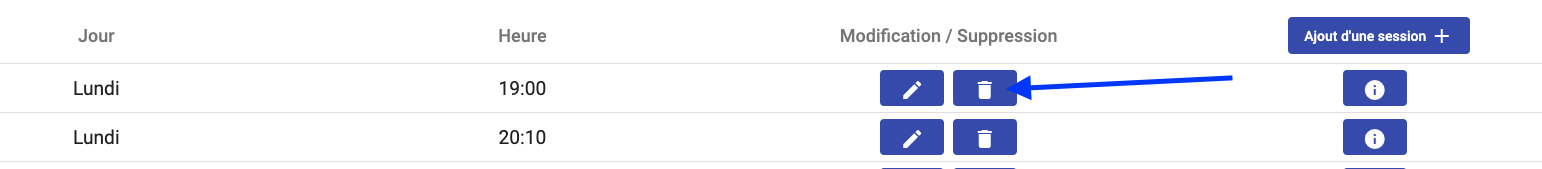
\includegraphics[width=0.9\textwidth,center]{Figures/us14-1}
	\caption{Bouton de suppression du type de session}
\end{figure}

\newpage
\begin{figure}[h]
	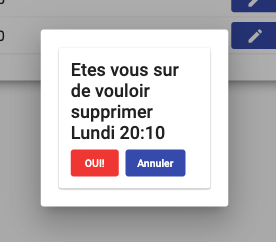
\includegraphics[width=0.4\textwidth,center]{Figures/us14-2}
	\caption{Fenêtre de confirmation de suppression}
\end{figure}

\subsubsection{Script concerné}
	\begin{itemize}
		\item \href{https://github.com/victorsmits/Aquabike/blob/master/backend/src/Controller/API/RegistrationControllerApi.php}{RegistrationControllerApi.php}
		\item \href{https://github.com/victorsmits/Aquabike/blob/master/backend/src/Entity/TypeSession.php}{TypeSession.php}
		\item \href{https://github.com/victorsmits/Aquabike/blob/master/frontend/src/app/type-session/del-type-session.component.ts}{del-type-session.component.ts}
		\item \href{https://github.com/victorsmits/Aquabike/blob/master/frontend/src/app/type-session/del-type-session.component.html}{del-type-session.component.html}
	\end{itemize}

	
	\vspace{\baselineskip}
	\vspace{\baselineskip}
	\subsection{En tant qu'administrateur, je veux pouvoir supprimer un utilisateur du système}
		\begin{enumerate}
	\item L'administrateur se connecte au site avec ses identifiants. 
	\item Un nouveau bouton de navigation apparait dans la barre de navigation. 
	\item L'administrateur clique sur le bouton \textit{Admin}
	\item Il sélectionne \textit{Abonnement} dans le menu déroulant. 
	\item L'administrateur atterrit sur la page de gestion des types des utilisateurs. 
	\item Il clique sur le bouton supprimer
	\item Une fenêtre de confirmation apparait. 
	\item Il clique sur \textit{OUI!} 
\end{enumerate}

\newpage
\begin{figure}[h]
	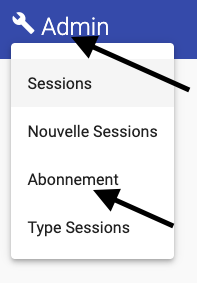
\includegraphics[width=0.4\textwidth,center]{Figures/us15-1}
	\caption{Menu de l'administrateur}
\end{figure}

\vspace{\baselineskip}
\begin{figure}[h]
	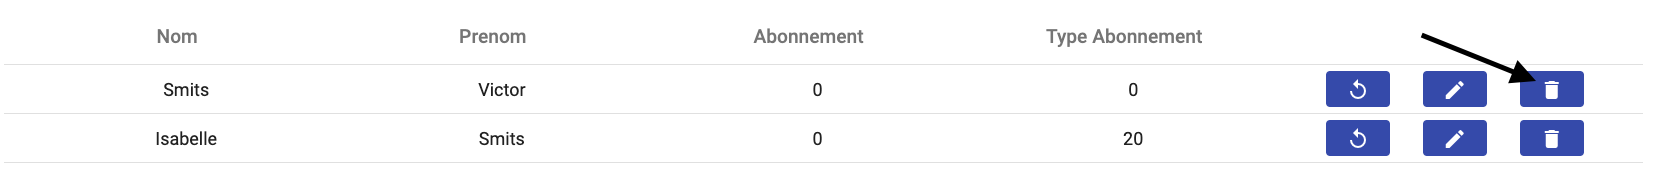
\includegraphics[width=\textwidth,center]{Figures/us15-2}
	\caption{Bouton de suppression de l'utilisateur}
\end{figure}

\vspace{\baselineskip}
\begin{figure}[h]
	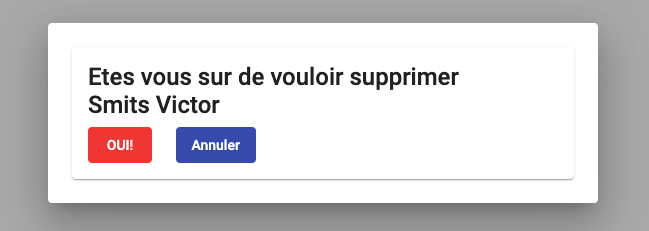
\includegraphics[width=0.5\textwidth,center]{Figures/us15-3}
	\caption{Fenêtre de confirmation de suppression}
\end{figure}

\subsubsection{Scripts concernés}
	\begin{itemize}
		\item \Href{https://github.com/victorsmits/Aquabike/blob/master/backend/src/Controller/API/AbonnementControllerApi.php}{AbonnementControllerApi.php}
		\item \Href{https://github.com/victorsmits/Aquabike/blob/master/backend/src/Entity/Person.php}{Person.php}
		\item \Href{https://github.com/victorsmits/Aquabike/blob/master/frontend/src/app/type-session/del-abo.component.ts}{del-abo.component.ts}
		\item \Href{https://github.com/victorsmits/Aquabike/blob/master/frontend/src/app/type-session/del-abo.component.html}{del-abo.component.html}
	\end{itemize}

	
	\newpage
	\subsection{En tant qu'administrateur, je dois pouvoir générer les sessions pour un nombre d'année}
		\begin{enumerate}
	\item L'administrateur se connecte au site avec ses identifiants. 
	\item Un nouveau bouton de navigation apparait dans la barre de navigation. 
	\item L'administrateur clique sur le bouton \textit{Admin}
	\item Il sélectionne \textit{Nouvelle session} dans le menu déroulant. 
	\item L'administrateur atterrit sur la page de création de session. 
	\item Il clique sur \textit{Génération auto}
	\item Un formulaire lui demandant sur combien d'années et le type de session il souhaite générer apparait.
	\item Il sélectionne les types de session qu'il souhaite générer.
	\item Il indique le nombre d'années voulus
	\item Il clique sur \textit{Je confirme la génération} 
\end{enumerate}

\vspace{\baselineskip}
\begin{figure}[h]
	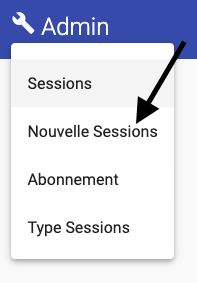
\includegraphics[width=0.4\textwidth,center]{Figures/us16-1}
	\caption{Menu de l'administrateur}
\end{figure}

\newpage
\begin{figure}[h]
	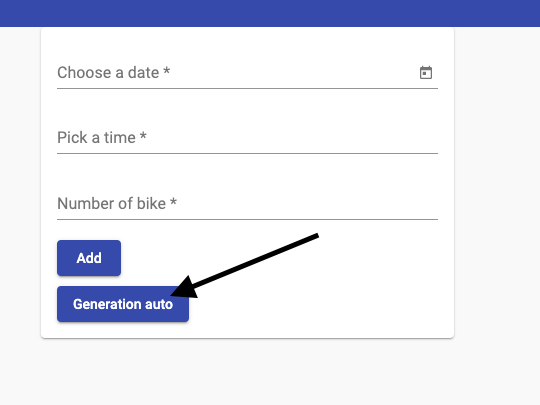
\includegraphics[width=0.4\textwidth,center]{Figures/us16-2}
	\caption{Bouton de génération automatique}
\end{figure}

\vspace{\baselineskip}
\begin{figure}[h]
	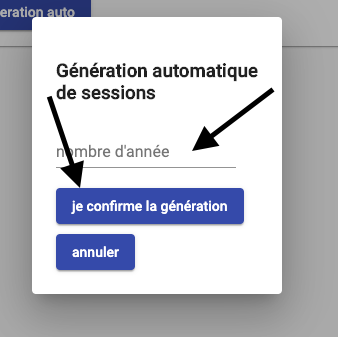
\includegraphics[width=0.3\textwidth,center]{Figures/us16-3}
	\caption{Formulaire pour la génération automatique de sessions}
\end{figure}


\subsubsection{Gestion des erreurs}
	\begin{itemize}
		\item La génération automatique suppose que tous les types de session on été préalablement configurés. Si ce n'est pas le cas, une erreur apparaitra à la confirmation.
		\item Si une erreur se crée durant la génération, elle est interrompue et un message d'erreur est affiché à l'administrateur.
	\end{itemize}
	
\newpage
\subsubsection{Diagramme de séquence}
	\begin{figure}[h]
		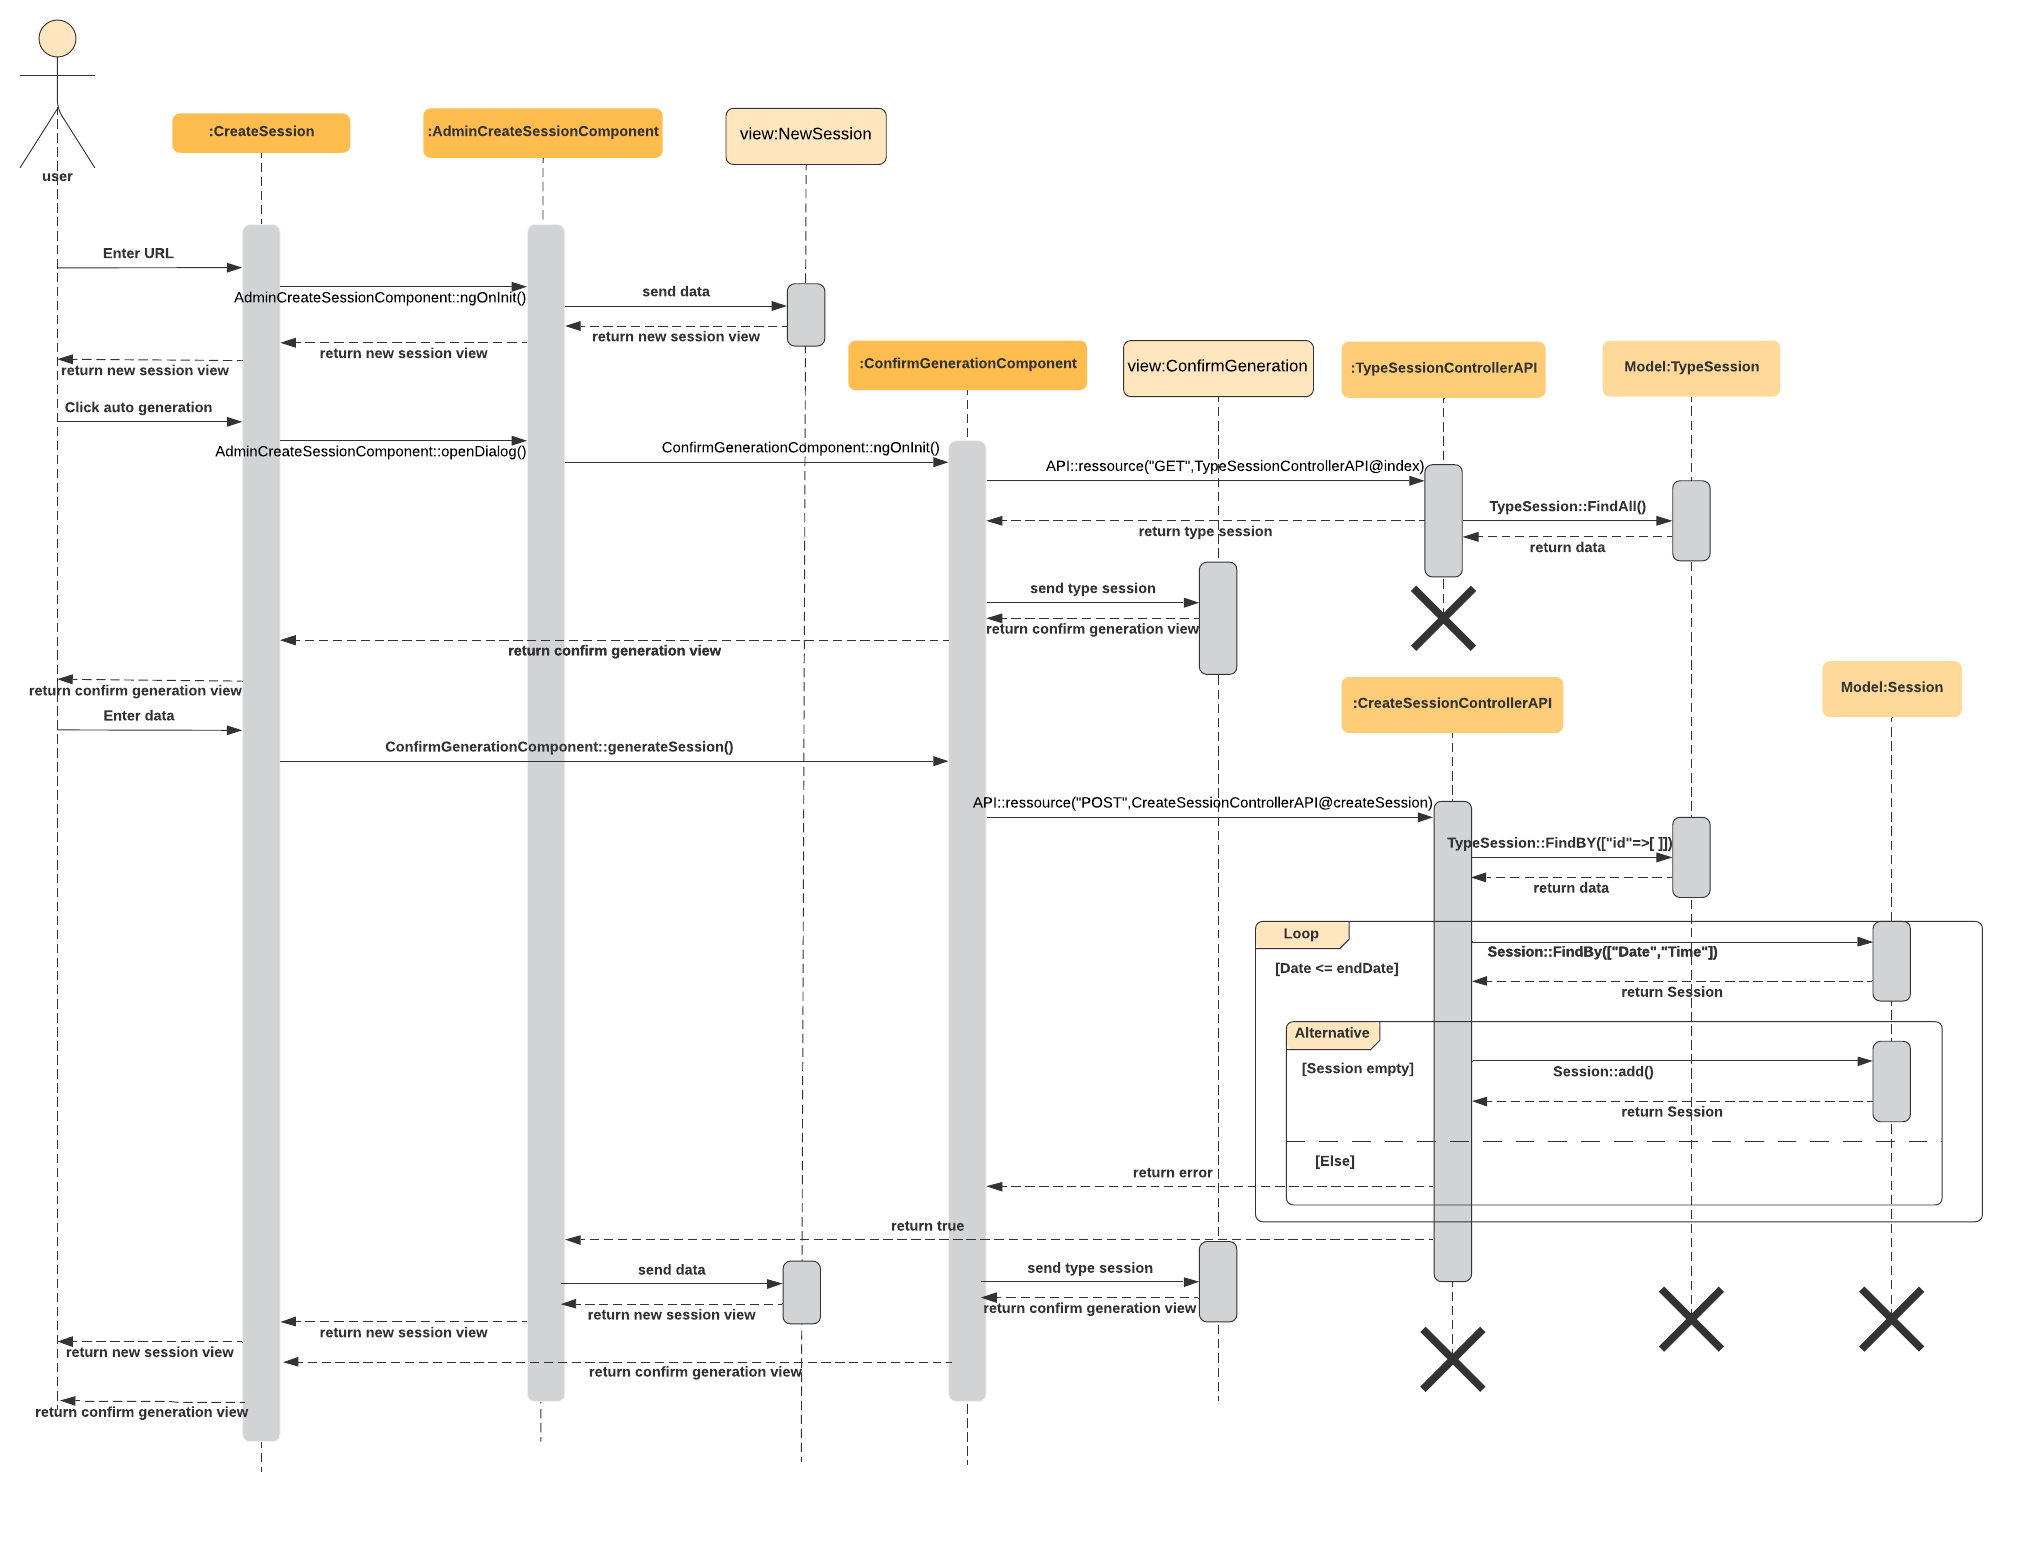
\includegraphics[width=\textwidth,center]{Diagramme/sequence-us16}
		\caption{Diagramme de séquence de la génération automatique de session}
	\end{figure}
	

\subsubsection{Scripts concernés}
	\begin{itemize}
		\item \Href{https://github.com/victorsmits/Aquabike/blob/master/backend/src/Entity/Session.php}{Session.php}
		\item \Href{https://github.com/victorsmits/Aquabike/blob/master/backend/src/Controller/API/CreateSessionControllerApi.php}{CreateSessionControllerApi.php}
		\item \Href{https://github.com/victorsmits/Aquabike/blob/master/frontend/src/app/admin-create-session/admin-create-session.component.ts}{admin-create-session.component.ts}
		\item \Href{https://github.com/victorsmits/Aquabike/blob/master/frontend/src/app/admin-create-session/admin-create-session.component.html}{admin-create-session.component.html}
	\end{itemize}

\newpage
\section{User Stories compatible Symfony-Angular}
	
	\subsection{En tant qu’utilisateur, je dois pouvoir me connecter sur le site}
		\subsubsection{Différences}
	\begin{itemize}
		\item Réalisation d'une requête POST via l'api REST permettant d'effectuer l'authentification dans le backend. 
		\item Différences au niveau de l'aspect graphique de la page de connection. 
		\item Connection via l'adresse Email et non le nom d'utilisateur. 
		\item Redirection automatique de l'utilisateur vers la page de connection lors de l'accès au site si l'utilisateur n'est pas connecté.
		\item Utilisation d'un LoginAuthenticator afin de pouvoir authentifier l'utilisateur dans le backend. 
		\item Utilisation de coockies pour préserver les informations de l'utilisateur. 
	\end{itemize}

\newpage
\subsubsection{Diagramme de séquence}
	\begin{figure*}[h!]
		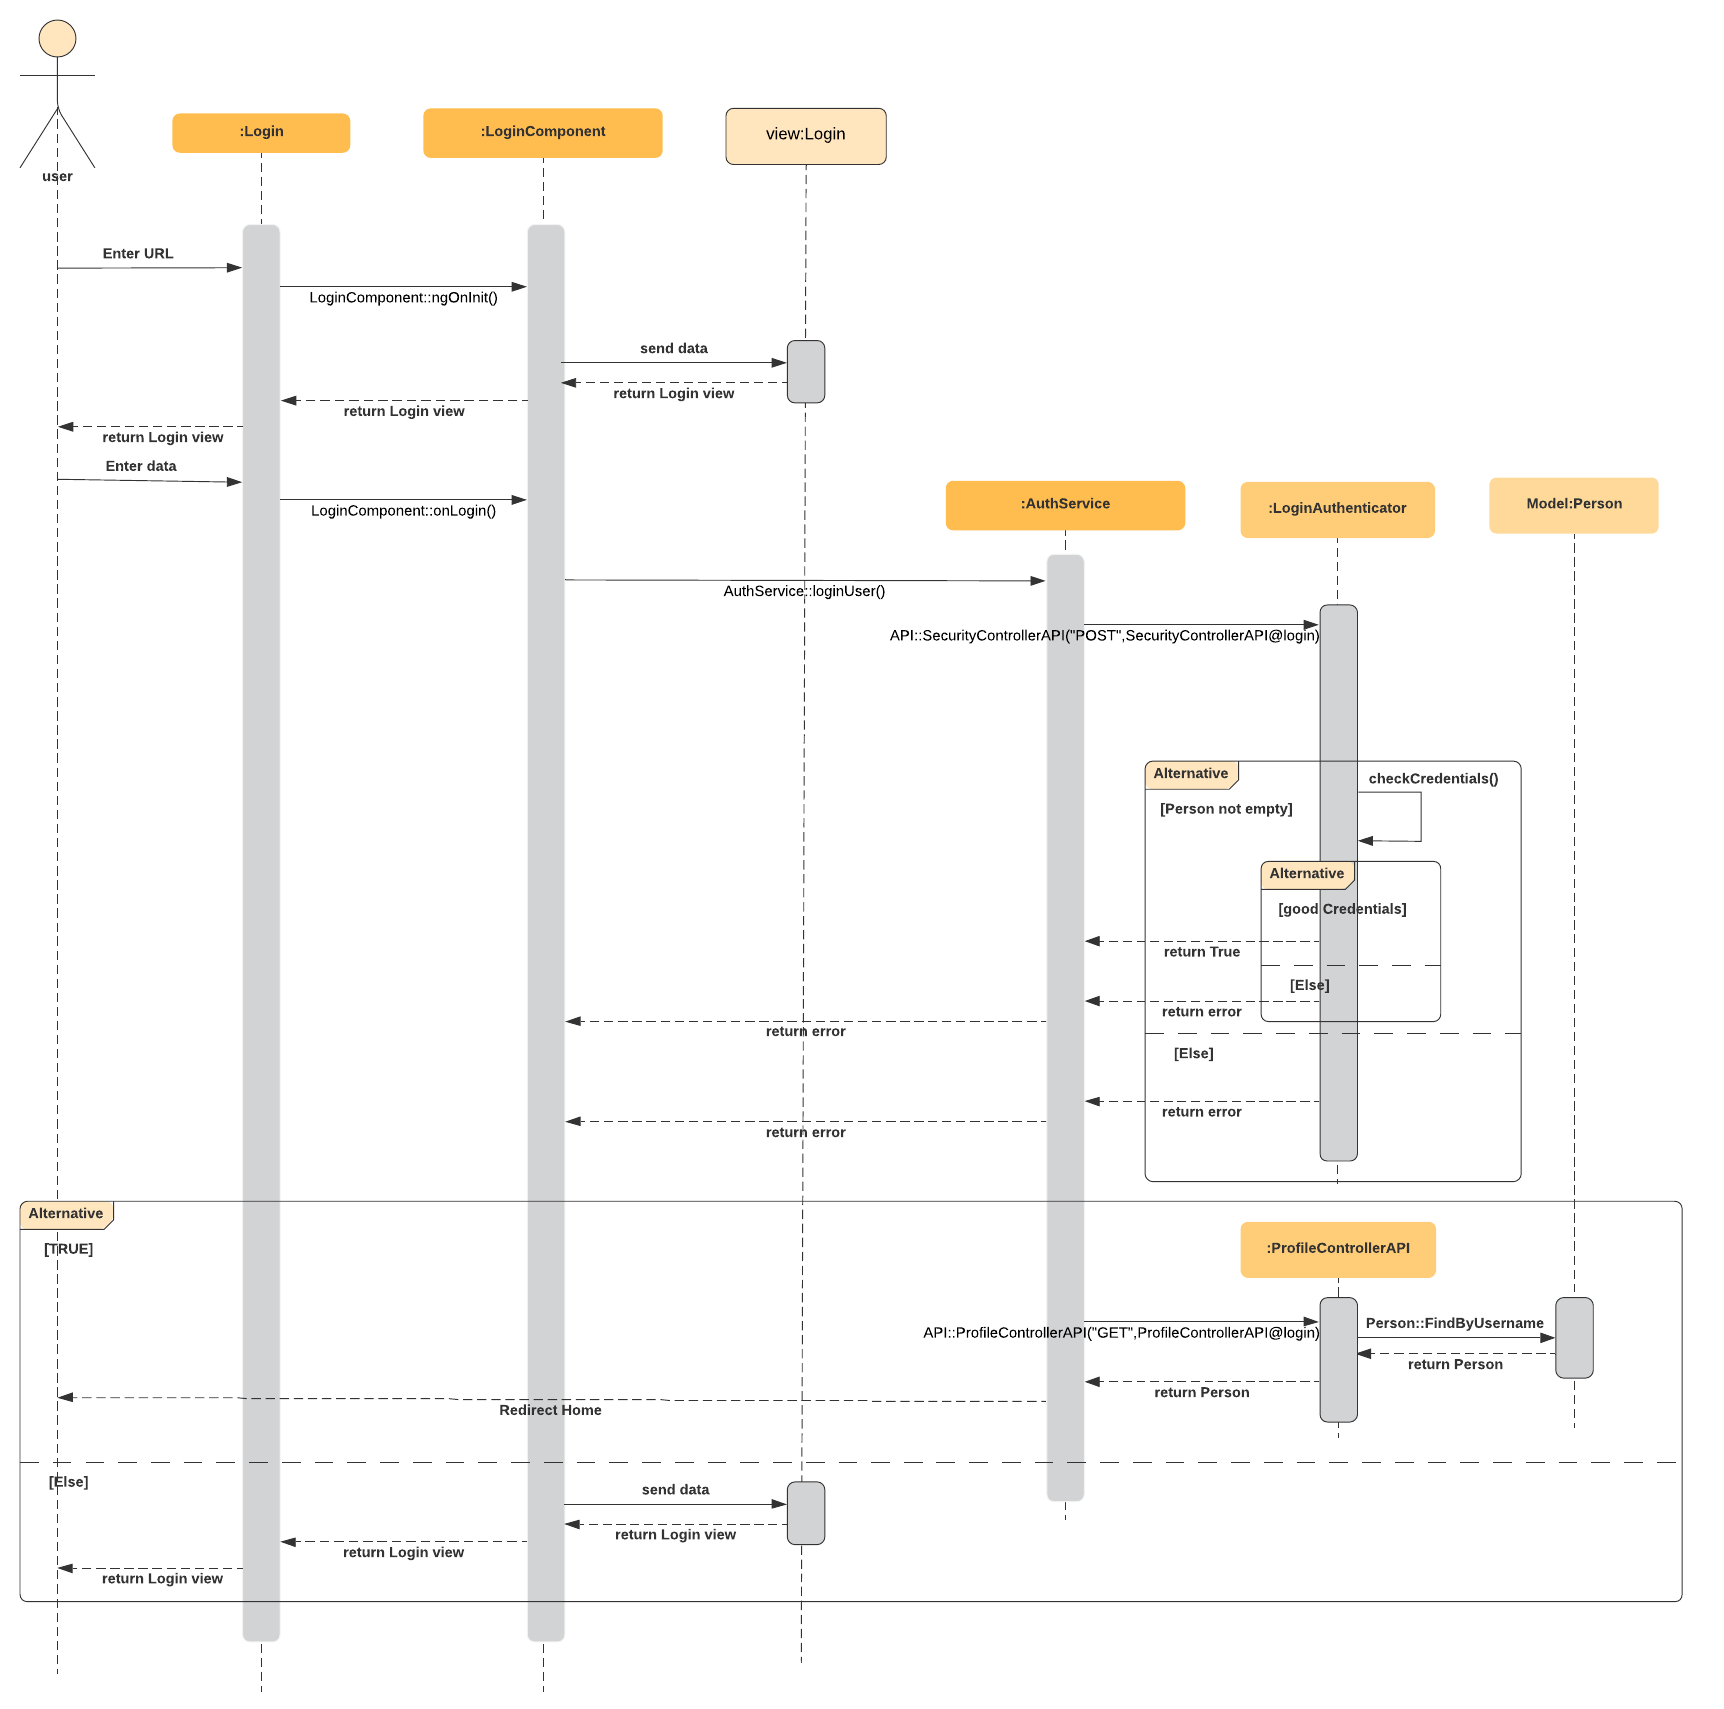
\includegraphics[width =\textwidth,center]{Diagramme/sequence-us0-angular}
		\caption{Diagramme de séquence de la connection d'un utilisateur}
	\end{figure*}

\newpage
\subsubsection{Scripts concernés}
	\begin{itemize}
		\item \Href{https://github.com/victorsmits/Aquabike/blob/master/frontend/src/app/service/api.service.ts}{api.service.ts}
		\item \Href{https://github.com/victorsmits/Aquabike/blob/master/frontend/src/app/service/auth.service.ts}{auth.service.ts}
		\item \Href{https://github.com/victorsmits/Aquabike/blob/master/backend/src/Controller/API/SecurityControllerAPI.php}{SecurityControllerAPI.php}
		\item \Href{https://github.com/victorsmits/Aquabike/blob/master/backend/src/Controller/API/ProfileControllerAPI.php}{ProfileControllerAPI.php}
		\item \Href{https://github.com/victorsmits/Aquabike/blob/master/frontend/src/app/login/login.component.ts}{login.component.ts}
		\item \Href{https://github.com/victorsmits/Aquabike/blob/master/frontend/src/app/login/login.component.html}{login.component.html}
		\item \Href{https://github.com/victorsmits/Aquabike/blob/master/backend/src/Entity/Person.php}{Person.php}
	\end{itemize}
	
	\newpage
	\subsection{En tant qu’utilisateur, je dois pouvoir me créer un compte sur le site}
		\begin{figure}[h]
	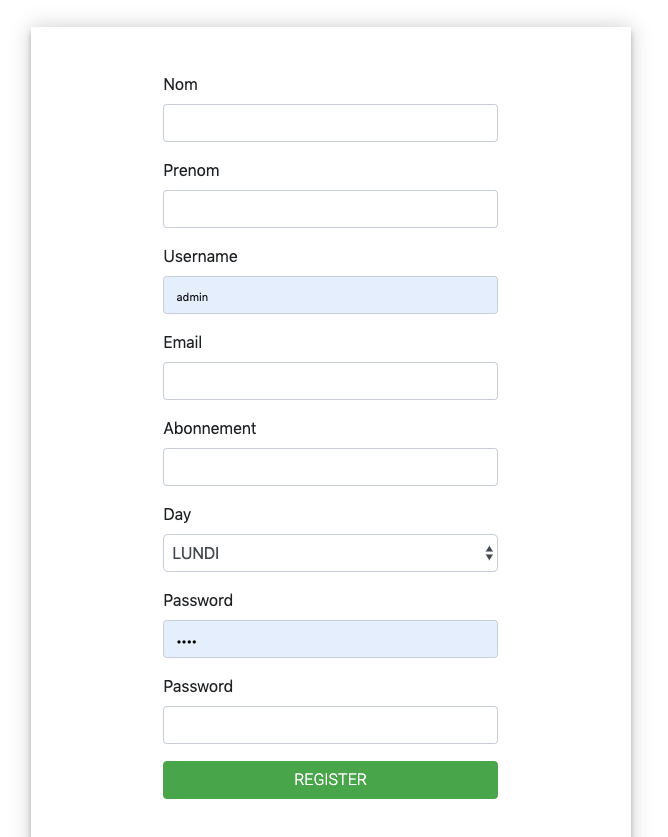
\includegraphics[width=0.5\textwidth,center]{Figures/us1-1}
	\caption{Formulaire d'inscription}
\end{figure}

\vspace{\baselineskip}
\begin{enumerate}
	\item L'utilisateur rentre ses information dans le formulaire. 
	\item L'utilisateur sélectionne le type de session à laquelle il est inscrit. 
	\item L'utilisateur clique sur \textit{Register} et attend la redirection. 
\end{enumerate}

\newpage
\subsubsection{Gestion des erreurs et sécurité}
	\paragraph{}
		\begin{itemize}
			\item L'utilisateur doit remplir tous les champs. Si un champ est manquant, une erreur apparaitra. 
			\item Le nom d'utilisateur et l'adresse Email sont uniques dans le système, s'il entre un Email ou nom d'utilisateur déjà existant, une erreur lui dira de corriger.
			\item L'utilisateur doit confirmer son mot de passe, si les mots de passe sont différents ou plus petits que 6 charactères il y aura un message d'erreur.
		\end{itemize}
		
\subsubsection{Diagramme de séquence}
	\begin{figure}[h]
		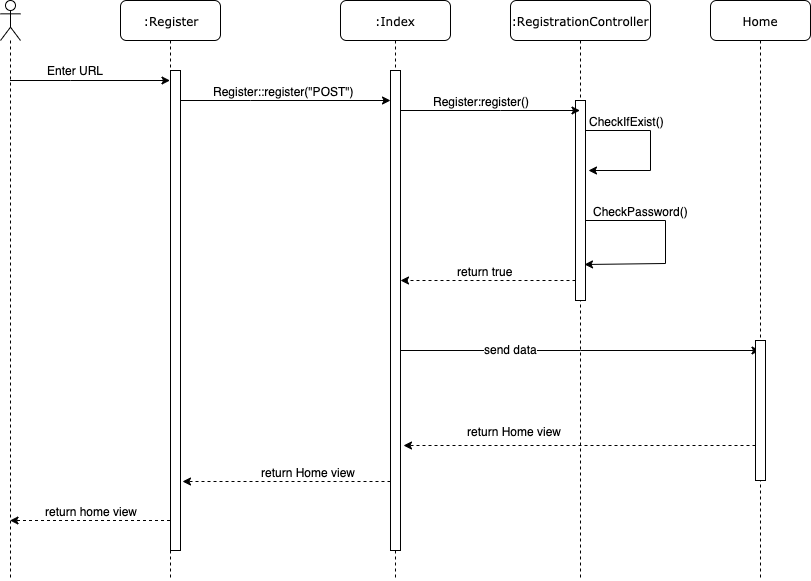
\includegraphics[width=0.8\textwidth,center]{Diagramme/sequence-us1}
		\caption{Diagramme de séquence de l'enregistrement d'un nouvelle utilisateur. }
	\end{figure}
	
	
\subsubsection{Scripts concernés}
	\begin{itemize}
		\item \Href{https://github.com/victorsmits/Aquabike/blob/master/backend/src/Controller/RegistrationController.php}{RegistrationController.php}
		\item \Href{https://github.com/victorsmits/Aquabike/blob/master/backend/templates/registration/register.html.twig}{register.html.twig}
		\item \Href{https://github.com/victorsmits/Aquabike/blob/master/backend/src/Entity/Person.php}{Person.php}
	\end{itemize}

	\vspace{\baselineskip}
	\subsection{En tant qu'utilisateur, je dois pouvoir sélectionner le mois et l'année pour afficher les sessions qui m'intéresse}
		\begin{figure*}[h]
	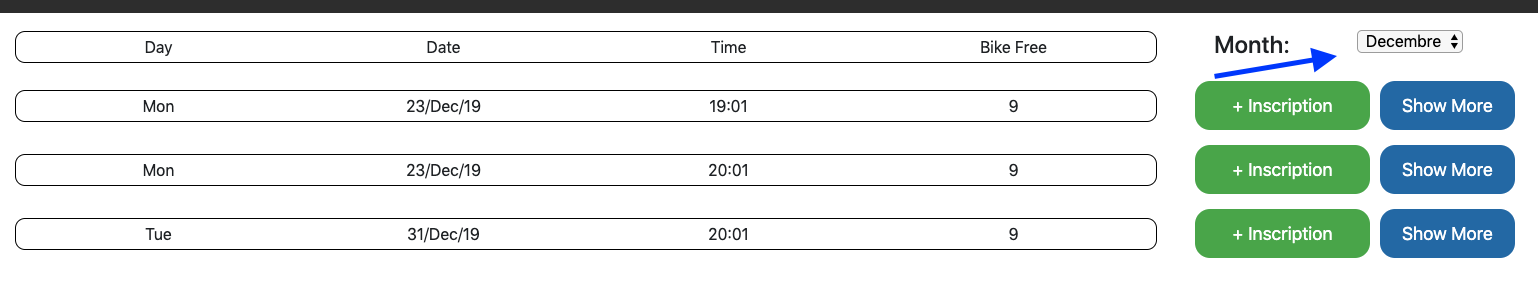
\includegraphics[width = 0.8\textwidth,center]{Figures/us2-1}
	\caption{selection du mois et de l'année}
\end{figure*}

\begin{enumerate}
	\item L'utilisateur choisit le mois et l'année. 
	\item la liste se rafraîchis afin de correspondre à la selection
\end{enumerate}
	
	\vspace{\baselineskip}
	\subsection{En tant qu’utilisateur, je dois pouvoir m’inscrire à une session un certain jour}
		\begin{figure*}[!h]
	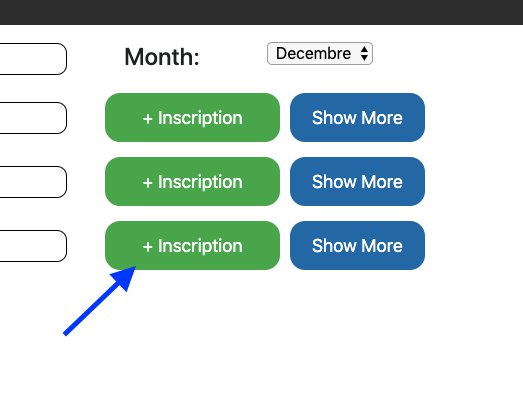
\includegraphics[width=0.5\textwidth,center]{Figures/us3-1}
	\caption{bouton d'inscritption}
\end{figure*}

\begin{enumerate}
	\item l'utilisateur choisit la session correspondant à sa demande.
	\item l'utilisateur clique sur le bouton  \textit{+ Inscription}
\end{enumerate}

\subsubsection{Gestion des erreurs}
	\begin{itemize}
		\item Si l'utilisateur ne possède plus d'abonnement, une erreur sera affichée lui signalant le problème. 
		\item Si la session est complète un message d'erreur sera affiché. 
	\end{itemize}
	
\subsubsection{Scripts concerné}
	\begin{itemize}
		\item \Href{https://github.com/victorsmits/Aquabike/blob/master/Symfony-Twig/src/Controller/MonthController.php}{MonthController.php}
		\item \Href{https://github.com/victorsmits/Aquabike/blob/master/Symfony-Twig/templates/month/month.html.twig}{month.html.twig}
		\item \Href{https://github.com/victorsmits/Aquabike/blob/master/Symfony-Twig/src/Entity/Session.php}{Session.php}
	\end{itemize}

	\vspace{\baselineskip}
	\subsection{En tant qu’utilisateur, je dois pouvoir être inscrit automatiquement à une session}
		\subsubsection{Différences}
	\begin{itemize}
		\item Réalisation de l'inscription automatique au session lors de l'enregistrement de l'utilisateurs. 
		\item Utilisation de type de session afin de facilité et de multiplier le choix des abonnements possible. 
		\item Possibilité pour un utilisateur de s'inscrire à plus de un type de session par semaine. 
		\item Sélection du type de session parmi une liste. 
	\end{itemize}

	\begin{figure*}[h!]
		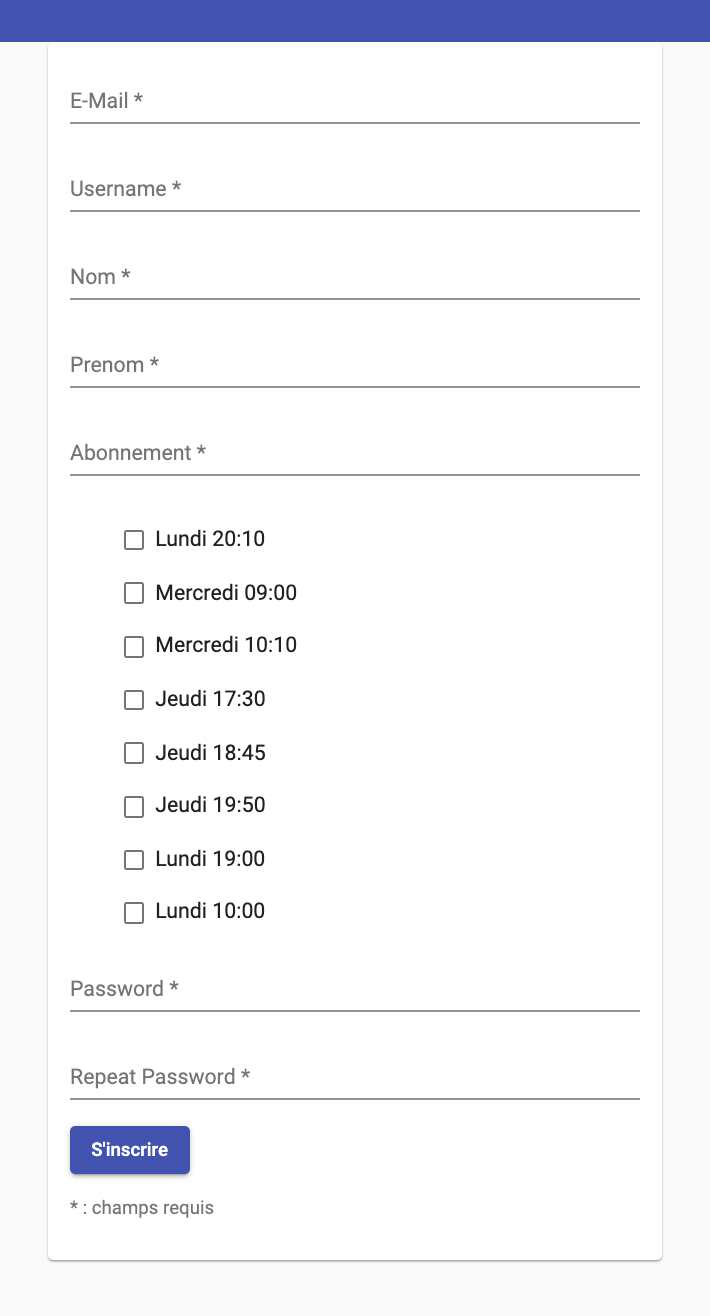
\includegraphics[width = 0.5\textwidth,center]{Figures/us4-1-angular}
		\caption{Formulaire d'inscription version angular}
	\end{figure*}
	
	
\newpage
\subsubsection{Diagramme de séquence}
	\begin{figure}[h]
		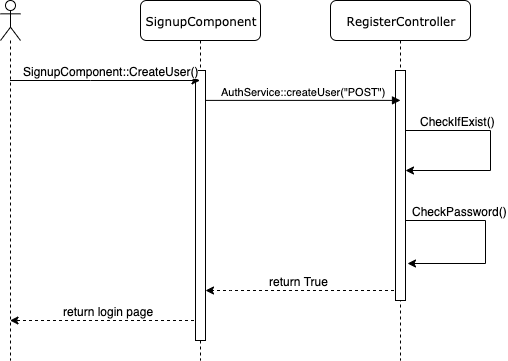
\includegraphics[width=\textwidth,center]{Diagramme/sequence-us1-angular}
		\caption{Diagramme de séquence de l'inscription automatique d'un utilisateur. }
	\end{figure}

\vspace{\baselineskip}
\subsubsection{Script concernés}
	\begin{itemize}
		\item \Href{https://github.com/victorsmits/Aquabike/blob/master/frontend/src/app/service/auth.service.ts}{auth.service.ts}
		\item \Href{https://github.com/victorsmits/Aquabike/blob/master/backend/src/Controller/API/SecurityControllerAPI.php}{SecurityControllerAPI.php}
		\item \Href{https://github.com/victorsmits/Aquabike/blob/master/backend/src/Entity/TypeSession.php}{TypeSession.php}
		\item \Href{https://github.com/victorsmits/Aquabike/blob/master/backend/src/Entity/Session.php}{Session.php}
		\item \Href{https://github.com/victorsmits/Aquabike/blob/master/backend/src/Entity/Inscription.php}{Inscription.php}
		\item \Href{https://github.com/victorsmits/Aquabike/blob/master/backend/src/Entity/Person.php}{Person.php}
		\item \Href{https://github.com/victorsmits/Aquabike/blob/master/frontend/src/app/signup/signup.component.ts}{signup.component.ts}
		\item \Href{https://github.com/victorsmits/Aquabike/blob/master/frontend/src/app/signup/signup.component.html}{signup.component.html}
	\end{itemize}
	
	\newpage
	\subsection{En tant qu’utilisateur, je dois pouvoir me désinscrire à une session}
		\begin{figure*}[h]
	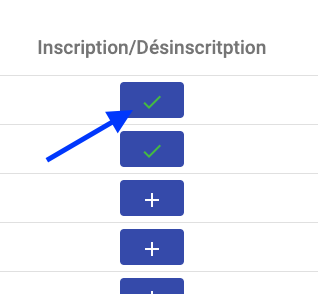
\includegraphics[width=0.5\textwidth,center]{Figures/us5-1}
	\caption{Bouton de désinscription à une session}
\end{figure*}

\begin{enumerate}
	\item L'utilisateur trouve la session qui l'interesse.
	\item Le check vert indique qu'il est inscrit.
	\item Il clique sur le bouton.
\end{enumerate}

\vspace{\baselineskip}
\subsubsection{Script concernés}
	\begin{itemize}
		\item \href{https://github.com/victorsmits/Aquabike/blob/master/backend/src/Controller/MonthController.php}{MonthController.php}
		\item \href{https://github.com/victorsmits/Aquabike/blob/master/backend/templates/registration/month.html.twig}{month.html.twig}
		\item \href{https://github.com/victorsmits/Aquabike/blob/master/backend/src/Entity/Person.php}{Person.php}
		\item \href{https://github.com/victorsmits/Aquabike/blob/master/backend/src/Entity/Inscription.php}{Inscription.php}
	\end{itemize}

	\vspace{\baselineskip}
	\subsection{En tant qu’utilisateur, je dois pouvoir voir qui est inscrit pour chaque session}
		\vspace{\baselineskip}
\begin{figure}[h]
	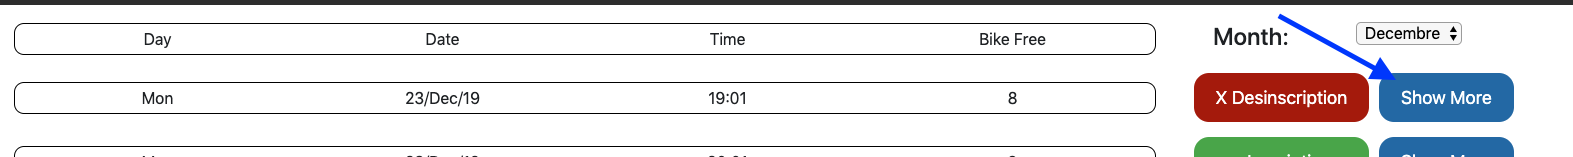
\includegraphics[width=0.9\textwidth,center]{Figures/us6-1}
	\caption{Bouton d'affichage}
\end{figure}

\begin{figure}[h]
	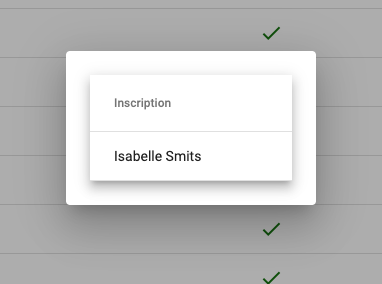
\includegraphics[width=0.5\textwidth,center]{Figures/us6-2}
	\caption{Liste Participant(e)s}
\end{figure}

\begin{enumerate}
	\item L'utilisateur trouve la session qui l'intéresse. 
	\item L'utilisateur clique sur le bouton information dans la colonne \textit{Liste Participant(e)s}. 
	\item Un tableau s'affiche avec la liste des inscrit(e)s. 
\end{enumerate}
	
	\newpage
	\subsection{En tant qu’utilisateur, je veux pouvoir voir dynamiquement le nombre de séance qui reste dans mon abonnement}
		\begin{enumerate}
	\item L'utilisateur clique sur son nom dans la bar de navigation.
	\item L'utilisateur est redirigé vers sa page de profil. 
	\item L'utilisateur retrouve l'information dans le cadre afficher sur la page.
\end{enumerate}

\vspace{\baselineskip}
\begin{figure}[h]
	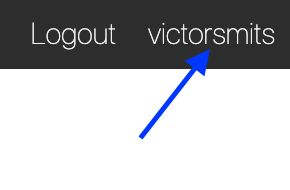
\includegraphics[width=0.5\textwidth,center]{Figures/us7-1}
	\caption{Bouton de navigation vers le profil}
\end{figure}

\vspace{\baselineskip}
\begin{figure}[h]
	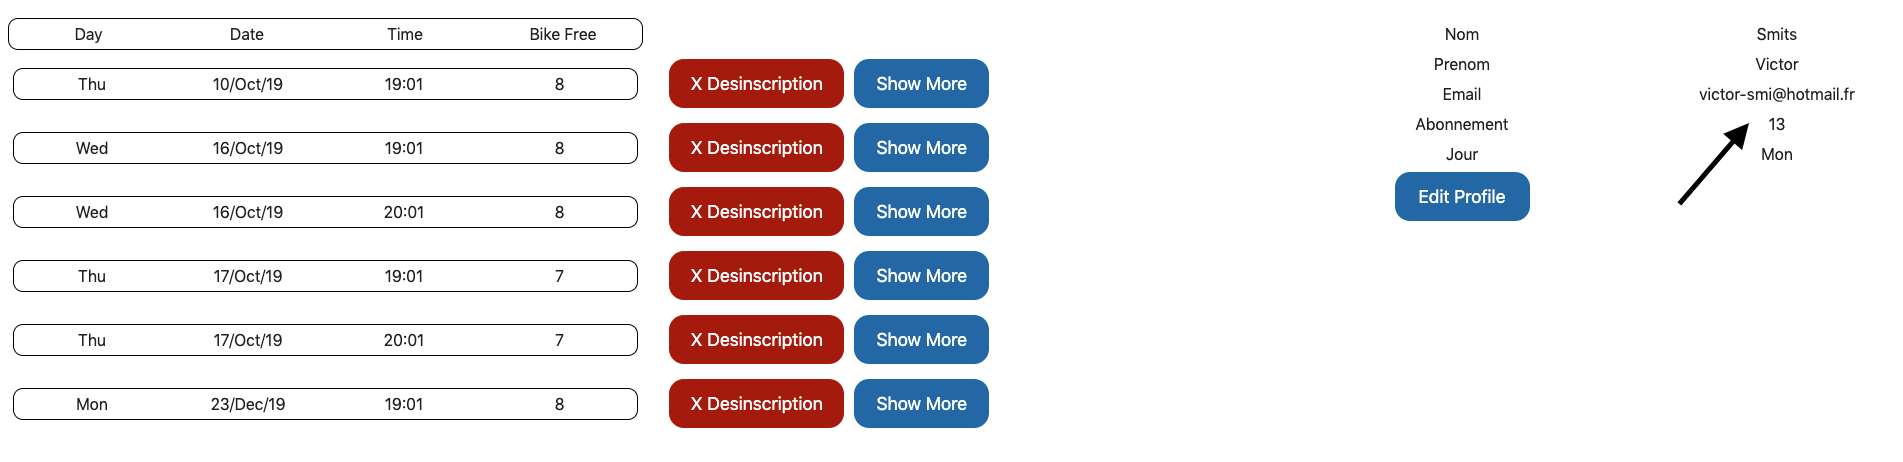
\includegraphics[width=0.9\textwidth,center]{Figures/us7-2}
	\caption{Nombre de séance restante dans l'abonnement}
\end{figure}


\vspace{\baselineskip}
\subsubsection{Script concernés}
	\begin{itemize}
		\item \Href{https://github.com/victorsmits/Aquabike/blob/master/backend/src/Controller/ProfileController.php}{ProfileController.php}
		\item \Href{https://github.com/victorsmits/Aquabike/blob/master/backend/templates/registration/profile.html.twig}{profile.html.twig}
		\item \Href{https://github.com/victorsmits/Aquabike/blob/master/backend/src/Entity/Person.php}{Person.php}
	\end{itemize}


	\newpage
	\subsection{En tant qu'utilisateur, je veux pouvoir modifier mon profile}
		\begin{enumerate}
	\item L'utilisateur clique sur son nom dans la bar de navigation.
	\item L'utilisateur clique sur \textit{Profil} dans le menu déroulant.
	\item L'utilisateur clique sur le bouton edit au dessus de son profil. 
	\item Une fenêtre apparait. 
	\item L'utilisateur rentre les information qu'il souhaite changer. 
	\item L'utilisateur confirm en cliquant sur \textit{ok}
\end{enumerate}

\vspace{\baselineskip}
\begin{figure}[h]
	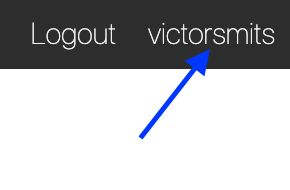
\includegraphics[width=0.4\textwidth,center]{Figures/us7-1}
	\caption{Bouton de navigation vers le profil}
\end{figure}

\begin{figure}[h]
	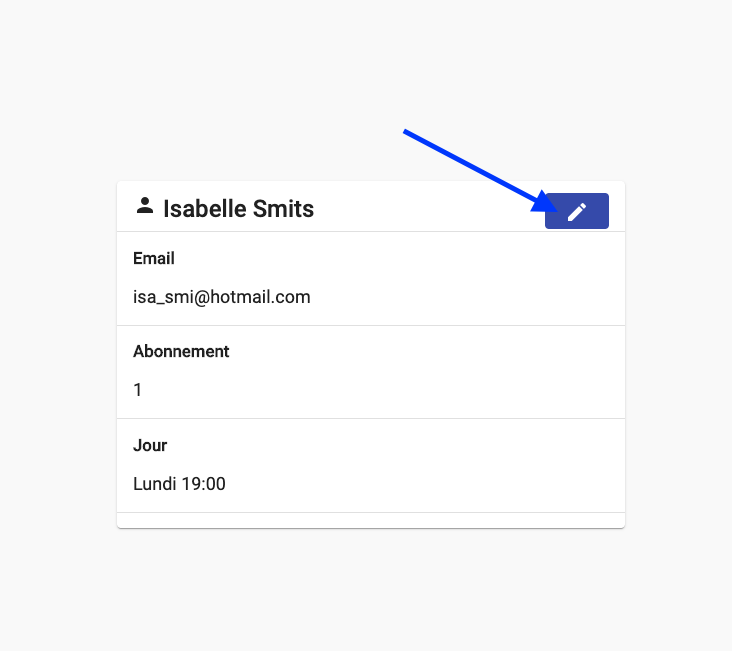
\includegraphics[width=0.4\textwidth,center]{Figures/us8-1}
	\caption{Bouton de modification du profil}
\end{figure}

\newpage
\begin{figure}[h]
	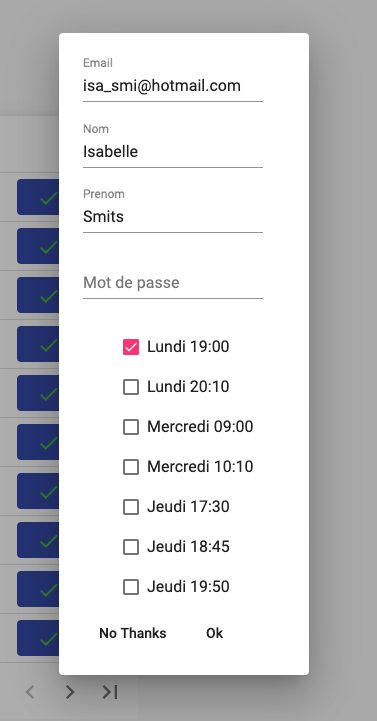
\includegraphics[width=0.4\textwidth,center]{Figures/us8-2}
	\caption{Fenêtre de modification des données du profil}
\end{figure}

	\newpage
	\subsection{En tant qu’administrateur, je dois pouvoir annuler une session}
		\subsubsection{Différences}
	\begin{itemize}
		\item Modification graphique du bouton d'annulation de la session. 
	\end{itemize}

\vspace{\baselineskip}
\subsubsection{Scripts concernés}
	\begin{itemize}
		\item \Href{https://github.com/victorsmits/Aquabike/blob/master/frontend/src/app/service/api.service.ts}{api.service.ts}
		\item \Href{https://github.com/victorsmits/Aquabike/blob/master/backend/src/Controller/API/SessionAdministrationControllerApi.php}{SessionAdministrationControllerApi.php}
		\item \Href{https://github.com/victorsmits/Aquabike/blob/master/backend/src/Entity/Session.php}{Session.php}
		\item \Href{https://github.com/victorsmits/Aquabike/blob/master/frontend/src/app/admin-session/admin-session.component.ts}{admin-session.component.ts}
		\item \Href{https://github.com/victorsmits/Aquabike/blob/master/frontend/src/app/admin-session/admin-session.component.html}{admin-session.component.html}
	\end{itemize}

	\vspace{\baselineskip}
	\subsection{En tant qu'administrateur, je dois pouvoir créer une nouvelle session peut importe la date}
		\subsubsection{Différence}
	\begin{itemize}
		\item Modification graphique du formulaire de création de session. 
	\end{itemize}
	
\vspace{\baselineskip}
\subsubsection{Script concernés}
	\begin{itemize}
		\item \href{https://github.com/victorsmits/Aquabike/blob/master/frontend/src/app/service/api.service.ts}{api.service.ts}
		\item \href{https://github.com/victorsmits/Aquabike/blob/master/backend/src/Controller/API/CreateSessionControllerApi.php}{CreateSessionControllerApi.php}
		\item \href{https://github.com/victorsmits/Aquabike/blob/master/backend/src/Entity/Session.php}{Session.php}
		\item \href{https://github.com/victorsmits/Aquabike/blob/master/frontend/src/app/admin-create-session/admin-create-session.component.ts}{admin-create-session.component.ts}
		\item \href{https://github.com/victorsmits/Aquabike/blob/master/frontend/src/app/admin-create-session/admin-create-session.component.html}{admin-create-session.component.html}
	\end{itemize}

	\vspace{\baselineskip}
	\vspace{\baselineskip}
	\subsection{En tant qu'administrateur, je dois pouvoir gérer les abonnement des utilisateurs}
		\subsubsection{Différence}
	\begin{itemize}
		\item Modification graphique de l'affichage des utilisateurs enregistré dans le système. 
	\end{itemize}

\vspace{\baselineskip}
\subsubsection{Script concernés}
	\begin{itemize}
		\item \href{https://github.com/victorsmits/Aquabike/blob/master/frontend/src/app/service/api.service.ts}{api.service.ts}
		\item \href{https://github.com/victorsmits/Aquabike/blob/master/backend/src/Controller/API/AbonnementControllerApi.php}{AbonnementControllerApi.php}
		\item \href{https://github.com/victorsmits/Aquabike/blob/master/backend/src/Entity/Person.php}{Person.php}
		\item \href{https://github.com/victorsmits/Aquabike/blob/master/frontend/src/app/admin-abo/admin-abo.component.ts}{admin-abo.component.ts}
		\item \href{https://github.com/victorsmits/Aquabike/blob/master/frontend/src/app/admin-abo/admin-abo.component.html}{admin-abo.component.html}
	\end{itemize}
